\section*{Conclusion}

\paragraph{}
Ce stage fût pour moi une grande opportunité. Il m'a permis de me rendre compte de la richesse des métiers du commerce international. Un grand marché est ouvert à ceux qui savent s'interfacer entre deux cultures. J'ai également découvert le milieu des très petites entreprises. Elles ont des avantages indéniables, facilité de communication, pouvoir se réinventer rapidement pour coller au plus proche des besoins. Leurs survies restent cependant dépendantes de la volonté des grandes entreprises. En discutant avec mes camarades en rentrant de stage, je m'aperçois de la diversité du milieu professionnel et des difficultés propres aux grandes entreprises. Je suis donc content d'avoir travaillé dans un cadre aussi amical.
 \paragraph{}
 Je souhaite à ProBespoke un développement fructueux. Cette entreprise a de nombreux atouts et elle devrait donc se démarquer dans ce marché. De mon côté j'espère pouvoir au cours de cette troisième année découvrir un milieu qui m'est encore inconnu celui de la recherche, peut-être encore à l'étranger si cela met proposer. Je partirais notamment deux mois en Russie cet octobre en échange avec l'Higher School of Economie de Moscou.
 \paragraph{}
\begin{figure}[h]
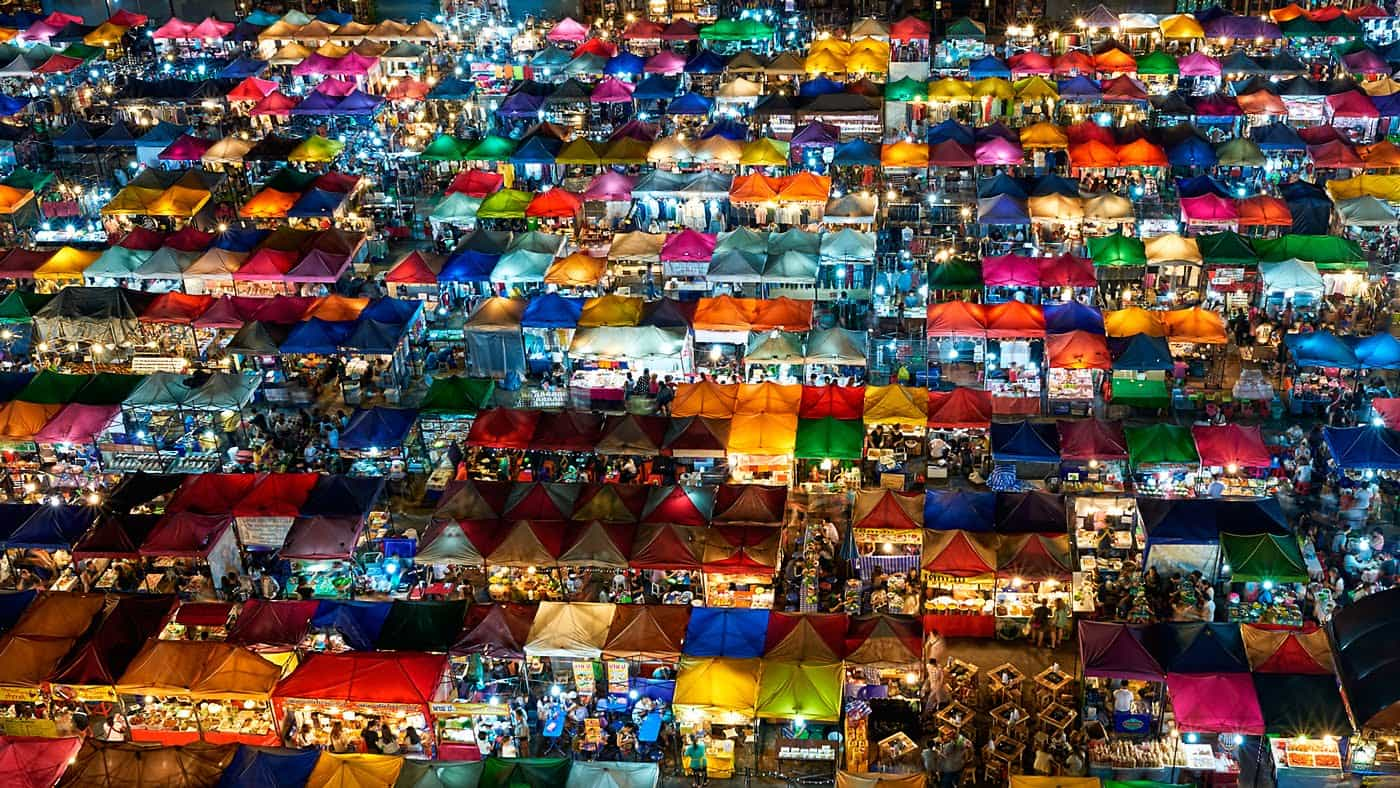
\includegraphics[width=16cm]{image/marche.jpg}
\caption{Un marché de nuit à Bangkok}
\end{figure}
